%% Based on a TeXnicCenter-Template by Tino Weinkauf.
%%%%%%%%%%%%%%%%%%%%%%%%%%%%%%%%%%%%%%%%%%%%%%%%%%%%%%%%%%%%%

%%%%%%%%%%%%%%%%%%%%%%%%%%%%%%%%%%%%%%%%%%%%%%%%%%%%%%%%%%%%%
%% HEADER
%%%%%%%%%%%%%%%%%%%%%%%%%%%%%%%%%%%%%%%%%%%%%%%%%%%%%%%%%%%%%
\documentclass[a4paper,twoside,10pt]{report}
% Alternative Options:
%	Paper Size: a4paper / a5paper / b5paper / letterpaper / legalpaper / executivepaper
% Duplex: oneside / twoside
% Base Font Size: 10pt / 11pt / 12pt


%% Language %%%%%%%%%%%%%%%%%%%%%%%%%%%%%%%%%%%%%%%%%%%%%%%%%
\usepackage[USenglish]{babel} %francais, polish, spanish, ...
\usepackage[T1]{fontenc}
\usepackage[ansinew]{inputenc}

\usepackage{lmodern} %Type1-font for non-english texts and characters


%% Packages for Graphics & Figures %%%%%%%%%%%%%%%%%%%%%%%%%%
\usepackage{graphicx} %%For loading graphic files
%\usepackage{subfig} %%Subfigures inside a figure
%\usepackage{tikz} %%Generate vector graphics from within LaTeX

%% Please note:
%% Images can be included using \includegraphics{filename}
%% resp. using the dialog in the Insert menu.
%% 
%% The mode "LaTeX => PDF" allows the following formats:
%%   .jpg  .png  .pdf  .mps
%% 
%% The modes "LaTeX => DVI", "LaTeX => PS" und "LaTeX => PS => PDF"
%% allow the following formats:
%%   .eps  .ps  .bmp  .pict  .pntg


%% Math Packages %%%%%%%%%%%%%%%%%%%%%%%%%%%%%%%%%%%%%%%%%%%%
\usepackage{amsmath}
\usepackage{amsthm}
\usepackage{amsfonts}


%% Line Spacing %%%%%%%%%%%%%%%%%%%%%%%%%%%%%%%%%%%%%%%%%%%%%
%\usepackage{setspace}
%\singlespacing        %% 1-spacing (default)
%\onehalfspacing       %% 1,5-spacing
%\doublespacing        %% 2-spacing


%% Other Packages %%%%%%%%%%%%%%%%%%%%%%%%%%%%%%%%%%%%%%%%%%%
%\usepackage{a4wide} %%Smaller margins = more text per page.
%\usepackage{fancyhdr} %%Fancy headings
%\usepackage{longtable} %%For tables, that exceed one page


%%%%%%%%%%%%%%%%%%%%%%%%%%%%%%%%%%%%%%%%%%%%%%%%%%%%%%%%%%%%%
%% Remarks
%%%%%%%%%%%%%%%%%%%%%%%%%%%%%%%%%%%%%%%%%%%%%%%%%%%%%%%%%%%%%
%
% TODO:
% 1. Edit the used packages and their options (see above).
% 2. If you want, add a BibTeX-File to the project
%    (e.g., 'literature.bib').
% 3. Happy TeXing!
%
%%%%%%%%%%%%%%%%%%%%%%%%%%%%%%%%%%%%%%%%%%%%%%%%%%%%%%%%%%%%%

%%%%%%%%%%%%%%%%%%%%%%%%%%%%%%%%%%%%%%%%%%%%%%%%%%%%%%%%%%%%%
%% Options / Modifications
%%%%%%%%%%%%%%%%%%%%%%%%%%%%%%%%%%%%%%%%%%%%%%%%%%%%%%%%%%%%%

%\input{options} %You need a file 'options.tex' for this
%% ==> TeXnicCenter supplies some possible option files
%% ==> with its templates (File | New from Template...).



%%%%%%%%%%%%%%%%%%%%%%%%%%%%%%%%%%%%%%%%%%%%%%%%%%%%%%%%%%%%%
%% DOCUMENT
%%%%%%%%%%%%%%%%%%%%%%%%%%%%%%%%%%%%%%%%%%%%%%%%%%%%%%%%%%%%%
\begin{document}

\pagestyle{empty} %No headings for the first pages.


%% Title Page %%%%%%%%%%%%%%%%%%%%%%%%%%%%%%%%%%%%%%%%%%%%%%%
%% ==> Write your text here or include other files.

%% The simple version:
\title{Estado del Arte}
\author{Federico Andrade \and Mart�n Llofri�}
%\date{} %%If commented, the current date is used.
\maketitle

%% The nice version:
%\input{titlepage} %%You need a file 'titlepage.tex' for this.
%% ==> TeXnicCenter supplies a possible titlepage file
%% ==> with its templates (File | New from Template...).


%% Inhaltsverzeichnis %%%%%%%%%%%%%%%%%%%%%%%%%%%%%%%%%%%%%%%
\tableofcontents %Table of contents
\cleardoublepage %The first chapter should start on an odd page.

\pagestyle{plain} %Now display headings: headings / fancy / ...



%% Chapters %%%%%%%%%%%%%%%%%%%%%%%%%%%%%%%%%%%%%%%%%%%%%%%%%
%% ==> Write your text here or include other files.


%\input{intro} %You need a file 'intro.tex' for this.


%%%%%%%%%%%%%%%%%%%%%%%%%%%%%%%%%%%%%%%%%%%%%%%%%%%%%%%%%%%%%
%% ==> Some hints are following:

\chapter{Introducci�n}

\section{Robots Aut�nomos}

Hoy en d�a, cada vez con m�s fuerza, la comunidad cient�fica al igual que la industria privada avanza en la b�squeda de robots que funcionen de forma aut�noma [ROOMBA],[DARPA CHALLENGE],[GOOGLE CAR]. En este sentido, uno de los principales problemas con los que tiene que se tiene que enfrentar un investigador o desarrollador de robots m�viles es el problemas de la localizaci�n. 
\\
\\
\begin{figure}[!hbt]
  \centering
    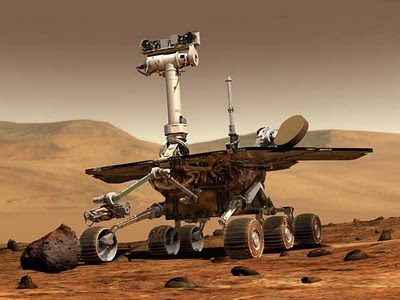
\includegraphics[width=0.5\textwidth]{images/oportunity.jpg}
  \caption{Imagen del robot Oportunity de la NASA en un entorno marciano}
  \label{fig:robotmovil}
\end{figure}

Existen muchas ocasiones en las que se conoce de antemano el entorno en el cual se mover� el robot y se le puede proporcionar un mapa del mismo. Un ejemplo podr�a ser un agente que siempre limpia la misma habitaci�n. N�tese que en este caso se debe realizar la tarea previa de crear un mapa.
\\
\\
Por otro lado hay situaciones en las que el agente rob�tico debe moverse en un entorno desconocido pero cuenta con informaci�n precisa sobre su ubicaci�n (en adelante \emph{pose}, compuesta por \emph{x} , \emph{y} y \emph{rotaci�n}). Para conocer su ubicaci�n se puede utilizar visi�n global o gps[SUMO, FUTBOLDEROBOTS], entre otras posibilidades. En este caso, el robot deber� arm�r un mapa del entorno apoyandose constantemente en la informaci�n de su ubicaci�n para tener mayores probabilidades de �xito.
\\
\\
Sin embargo, existes casos, a�n m�s complejos que los mencionados, en los que no se conoce el entorno y tampoco se tiene informaci�n sobre la ubicaci�n exacta del robot. En este caso el robot deber� generar un mapa y mantener su ubicaci�n en el mismo, todo a la vez. Esta tarea resulta compleja por el hecho que para poder localizarse de forma precisa se necesita un mapa y por otro lado, para poder crear un mapa es menester estar localizado en forma precisa. Esta es la tarea que estudia el SLAM, localizaci�n y armado de mapas simultaneo. Algunos ejemplos en los cuales es importante realizar SLAM son:

%poner mas ejemplos
\begin{itemize}
	\item exploraci�n espacial
	\item rescate en zonas modificadas por cat�strofes
	\item robots que realizan tareas dom�sticas
	\item autos dirigidos de forma aut�noma
\end{itemize}



\section{El problema del SLAM}

El problema del SLAM (en espa�ol: Localizaci�n y armado de mapas simultaneo) comienza cuando el robot no tiene acceso a un mapa del entorno y tampoco conoce su pose en el mismo. El robot solamente posee medidas \begin{math}z_{1:t}\end{math} obtenidas de los sensores y controles \begin{math}u_{1:t}\end{math} con los cuales puede actuar sobre el ambiente. El agente intentar� obtener un mapa del entorno y simultaneamente localizarse relativo a dicho mapa[handbook].
\\
\\

\begin{figure}[!hbt]
  \centering
    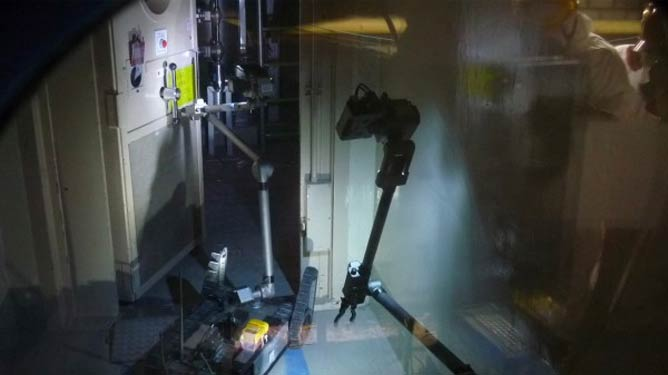
\includegraphics[width=0.5\textwidth]{images/irobotjapon.jpg}
  \caption{Robot de la empresa IRobot realizando un rescate en un �rea de cat�strofe}
  \label{fig:irobotjapon}
\end{figure}

En la actualidad existen m�todos de SLAM robustos para mapear ambientes est�ticos, estructurados y de tama�o limitado. Realizar SLAM en entornos din�micos, espacialmente grandes y desestructurados sigue siendo un problema abierto a la investigaci�n.
%no se a que se refiere el libro con estructurados. Supongo que habla de ambientes con paredes y cajas en lugar de
%ambiente con piedras totalmente irregulares, pero no estoy seguro, sino lo sacamos

\section{Desaf�os}

A continuaci�n se presentan los principales desaf�os que tiene el problema del SLAM.

\subsection{Incertidumbre}

Como se mencion� anteriormente, determinar la posici�n exacta del robot requiere conocimiento sobre la posici�n exacta de 
%no se dijo nada aun de que el entorno se ve como un conjunto de caracteristicas
las caracter�sticas del entorno. Por otro lado, la determinaci�n de la posici�n exacta de las caracter�sticas del entorno requiere conocimiento de la posici�n exacta del agente. Dado que el agente no posee inicialmente ninguno de estos datos, y dado que la incertudimbre de su posici�n aumenta con su movimiento, el algoritmo de SLAM debe ser capaz de manejar cierto error en los datos que son computados.
\\
\\
\begin{figure}[!hbt]
  \centering
    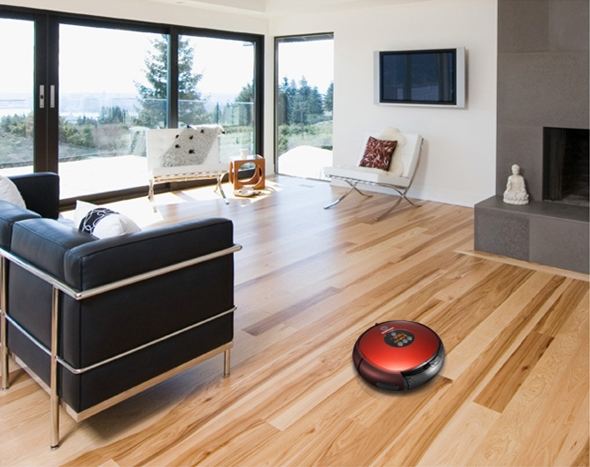
\includegraphics[width=0.5\textwidth]{images/navibot.jpg}
  \caption{Imagen de un robot m�vil situado en una posici�n inicial desconocida y en un ambiente desconocido}
  \label{fig:slam}
\end{figure}

Esta incertidumbre debe ser manejada de forma tal que el error en las estimaciones no crezca constantemente (de manera de evitar una divergencia en la estimaci�n de la posici�n del robot y las caracter�sticas de su entorno).

\subsection{Sensores}

Los sensores son limitados en lo que pueden percibir y poco precisos en sus medidas. Estas limitaciones vienen dadas por muchos factores. El rango y la resoluci�n de un sensor est� sujeto a limitaciones f�sicas. Un claro ejemplo son las c�maras cuya calidad de im�gen es limitada. Los sensores adem�s est�n sujetos a ruido estoc�stico, lo que perturba las medidas de formas impredecibles y hace que la informaci�n extra�da sea poco confiable. Otro problema que incrementa el ruido en los sensores es el hecho de realizar medidas con el robot en movimiento, hecho que genera mayor error en las medidas de los sensores.
\\
\\
\begin{figure}
  \centering
    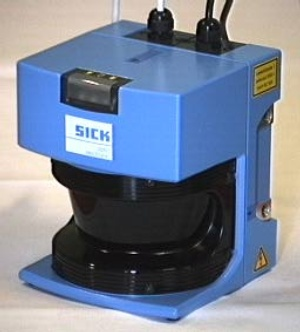
\includegraphics[width=0.5\textwidth]{images/sick.jpg}
  \caption{Sensor laser comunmente utilizado para hacer SLAM}
  \label{fig:sensor}
\end{figure}

Finalmente, lo sensores pueden sufrir da�os, y detectar una falla de este tipo puede ser extremadamente dif�cil.



\subsection{Controles}

En la fase de exploraci�n del SLAM (sea activo o pasivo, ver \ref{activovspasivo}) se env�an ordenes de movimiento al robot, conocidos como controles. Una vez que se le envia una orden de movimiento al robot, los sensores en los motores (odometr�a) permiten conocer cual ha sido el movimiento que hizo el robot a partir de la orden que fue solicitada. Esta informaci�n luego se procesar� para actualizar la posici�n del robot. El problema ocurre cuando una de las ruedas del robot queda en el aire o simplemente resbala sobre una superficie con baja adeherencia lo que implica que el robot no cambi� su posici�n, o lo hizo pero en menor medida de la esperada, sin embargo los datos devueltos por los sensores de odometr�a indican que el movimiento fue completo. Esto genera un error entre la pose real del robot y su creencia de la posici�n.

\begin{figure}[!hbt]
  \centering
    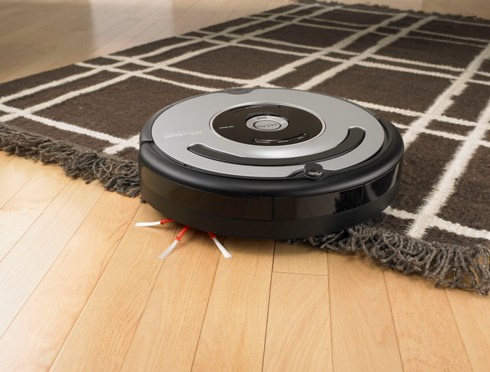
\includegraphics[width=0.5\textwidth]{images/roomba.jpg}
  \caption{Imagen de un robot utilizado para limpieza dom�stica subiendo una alfombra, caso t�pico de quedar con una rueda en el aire o patinar}
  \label{fig:roomba}
\end{figure}

\subsection{Ciclos}

Cerrar ciclos quiere decir que el robot debe poder reconocer cuando pasa por un lugar que ya ha sido visitado. Realizar esta tarea con �xito se vuelve primordial en los mapas que poseen muchos cruces.

\begin{figure}[!hbt]
  \centering
    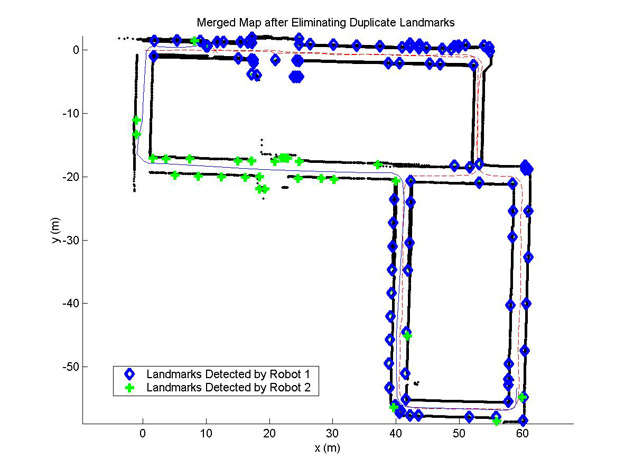
\includegraphics[width=0.5\textwidth]{images/loopclosure.jpg}
  \caption{T�pico escenario de pruebas donde el robot deber� tener un buen sistema para cerrar ciclos}
  \label{fig:loop}
\end{figure}

\subsection{Asociaci�n incorrecta}

El agoritmo de SLAM debe ser lo suficientemente robusto como para no confundir dos lugares diferentes de forma que lo lleve a creer ques son el mismo. En caso de que el robot piense que dos lugares diferentes con caracter�sticas similares son efectivamente el mismo, cerrar� un ciclo donde no lo hay y generar� un mapa incorrecto del entorno lo cual puede llevar a errores catastr�ficos.

\subsection{Capacidad de c�mputo}

Una gran limitaci�n del SLAM es el procesamiento. Los algor�tmos de SLAM suelen realizar tareas de procesamiento pesadas debido a la cantidad de caracter�sitcas del ambiente que manejan (que suelen incrementarse con el paso del tiempo), el mapa y la estimaci�n de la posici�n. Esto muchas veces hace dificil el procesamiento dentro del robot y obliga a extraer los datos sensados para ser procesados afuera.


\section{Clasificaciones de SLAM} %esto es parte del problema o de la solucion?

Los problemas de SLAM se mueven sobre muchas dimensiones diferentes. Los art�culos m�s importantes identifican los tipos de problemas definiendo en cual de estas dimensiones trabajan. A continuaci�n presentamos las distinciones m�s importantes sobre el problema del SLAM.

\subsection{Full vs. Online}

Desde el punto de vista probabil�stico existen dos enfoques del problema del SLAM. Uno de ellos es el Online SLAM que se trata de la estimaci�n de la posterior %(explicar q es esto)
basado en la posici�n actual
\\
\\
\begin{math}
	\Pr(x_t, m \mid z_{1:t}, u_{1:t})
\end{math}
\\
\\
Donde \begin{math}x_t\end{math} es la pose en el tiempo t, m es el mapa y \begin{math}z_{1:t}\end{math} y \begin{math}u_{1:t}\end{math} son las medidas obtenidas de los sensores y los controles respectivamente. Muchos algoritmos de online SLAM son incrementales, es decir que descartan medidas anteriores una vez que fueron procesadas.

En el caso del full SLAM se busca calcular la posterior sobre todas las posiciones anteriores \begin{math}x_{1:t}\end{math} en el mapa, en lugar de utilizar solamente la posici�n actual \begin{math}x_t\end{math}.
\\
\\
\begin{math}
	\Pr(x_{1:t}, m \mid z_{1:t}, u_{1:t})
\end{math}
\\
\\
En la pr�ctica, realizar full SLAM es inviable.

\subsection{Offline vs. Online}

En el caso del SLAM online se procesa la informaci�n en el mismo robot mientras este navega en el entorno. Por otro lado, en el offline se realiza SLAM sobre un conjunto de datos que previamente fueron recuperados con alg�n robot, tanto de la medida de sus sensores como las medidas de odometr�a (movimiento).  

\subsection{Topol�gico vs. M�trico}

Algunas t�cnicas de armado de mapas solamente mantienen la descripci�n de algunas caracter�sticas del entorno, que caracteriza la relaci�n entre lugares. Estos m�todos son conocidos como topol�gicos. Un mapa topol�gico se define por un conjunto de lugares diferentes y otro conjutno que caracterizan las relaciones entre estos. Por otro lado, los m�todos m�tricos proveen informaci�n m�trica entre los lugares. En los �ltimos a�os los m�todos topol�gicos han pasado de moda apesar de la amplia evidencia de que los humanos utilizan a menudo informaci�n topol�gica. 

\subsection{Activo vs. Pasivo}\label{activovspasivo}

En los algoritmos de SLAM pasivos es otra entidad quien se encarga de controlar el robot, mientras que el algoritmo pasivo es puramente observador. La gran mayor�a de los algoritmos de SLAM son de este tipo. En el caso de los algoritmos activos, el robot explora de forma activa en entorno en busca de conseguir un mapa mas preciso en el menor tiempo posible. Existen t�cnicas hibridas donde el algoritmo de SLAM solo controla la direcci�n de los sensores y otra entidad se encarga de la direcci�n del movimiento del robot.

\subsection{Est�tico vs. Din�mico}

En el caso del SLAM est�tico se asume que el entorno no cambia con el tiempo a diferencia de los m�todos din�micos que s� lo hacen. La gran mayor�a de la literatura asume entornos est�ticos. 


\subsection{Volum�trico vs. Basado en marcas}

En SLAM volum�trico, el mapa es muestreado a una resoluci�n que permite una reconstrucci�n fotogr�fica del entorno. En este caso el costo computacional es alto. Por otro lado, en el SLAM basado en marcas se extraen caracter�sticas de las medidas de los sensores de forma de armar el mapa en base a caracter�sticas dispersas. Las t�cnicas que utilizan SLAM basado en marcas suelen ser mas eficientes ya que se descarta informaci�n de los sensores. 

\subsection{Correspondencia conocida vs. Desconocida}

El problema de correspondencia es el problema de realacionar la identidad de marcas sensadas en el pasado con marcas sensadas actualmente. Algunos algoritmos de SLAM asumen que la correspondencia es conocida, esto implica que cuando se est� midiendo una marca alguna entidad provee al n�cleo del SLAM la informaci�n de que marca es la que se est� midiendo. Los algoritmos que no asumen la correspondencia proveen mecanismos para estimar la correspondencia de las medidas con las marcas previamente observadas en el mapa. El problema de estimar la correspondencia es conocido como \it{problema de asociaci�n de datos}, y es uno de los m�s dif�ciles en el SLAM.

\subsection{SLAM con un solo robot vs. Multirobot}

La gran parte de los problemas est�n definidos para un solo robot, sin embargo, recientemente el problema de trabajar con m�s de un robot ha ganado mucha popularidad. Los problemas para multirobots vienen de muchas maneras. En algunos casos los robots son capaces de observarse entre ellos, mientras que otros no. Tambi�n se distinguen por el tipo de comunicaci�n que utilizan. Los m�s realistas permiten que solamente los robots que estan m�s cerca se puedan comunicar entre ellos.

\subsection{Manejo de mucha incertidumbre vs. poca incertidumbre}

Estos algoritmos se distinguen por la cantidad de incertidumbre que pueden manejar. Los m�s simples solo pueden manejar poca incertidumbre en la localizaci�n. Son �tiles para los casos en los cuales un camino no se intersecta a s� mismo. En cambio para los mapas los cuales tienen lugares que se pueden alcanzar de muchas maneras (ver \ref{fig:loop}) es necesario que el robot pueda manejar mucha incertidumbre en su posici�n. La incertidumbre puede ser disminuida si el robot puede sensar informaci�n sobre su posici�n de forma absoluta. Un ejemplo puede ser mediante el uso sistema de posicionamiento global (GPS).%intro

\chapter{T�cnicas aplicadas en SLAM} 

\section{Filtros de Kalman} 

\section{Part�culas} 

\section{Grafos} 
%tecnicas

\chapter{Subproblemas} 

% Esta seccion va a ser fruta
\section{Enfoques} 

\subsection{Bioinspirados} 
% leer un par de reviews
\subsection{Probabil�sticos} 
% Bayes (modelos bayesinos), estado oculto, marcov (marcov assumption), HMM

\section{Modelo de sensado}

\section{Modelo de movimiento}

\section{Representaci�n del mapa}
\subsection{Grillas de ocupaci�n}


\section{Prcesamiento de la informaci�n}
% ruido, filtros, estimacion continua, estimador optimador, problema de dimensionalidad (aumento con el paso del tiempo), unimodal, multimodal (para despues capaz). 

\subsection{Filtros de Kalman} 

\subsection{Part�culas} 

\subsection{Grafos} %tipos de slam

\chapter{Casos de estudio}

\section{FastSLAM}
%casos de estudio

\chapter{Ejemplo}\label{hints}%este lo dejo de ejemplo, pero hay q pelarlo en el futuro

\section{German Umlauts and other Language Specific Characters}\label{umlauts}
You can type german umlauts like '�', '�', or '�' directly in this file.
This is also true for other language specific characters like '�', '�' etc.

There are problems with automatic hyphenation when using language
specific characters and OT1-encoded fonts. In this case, use a
T1-encoded Type1-font like the Latin Modern font family (\verb#\usepackage{lmodern}#).


\section{References}\label{references}
Using the commands \verb#\label{name}# and \verb#\ref{name}# you are able
to use references in your document. Advantage: You do not need to think
about numerations, because \LaTeX\ is doing that for you.

For example, in section \ref{dividing} on page \pageref{dividing} hints for
dividing large documents are given.

Certainly, references do also work for tables, figures, formulas\ldots

Please notice, that \LaTeX\ usually needs more than one run (mostly 2) to
resolve those references correctly.


\section{Dividing Large Documents}\label{dividing}
You can divide your \LaTeX-Document into an arbitrary number of \TeX-Files
to avoid too big and therefore unhandy files (e.g. one file for every chapter).

For this, you insert in your main file (this one) for every subfile
the command '\verb#\input{subfile}#'. This leads to the same behavior
as if the content of the subfile would be at the place of the \verb#\input#-Command.


%% <== End of hints
%%%%%%%%%%%%%%%%%%%%%%%%%%%%%%%%%%%%%%%%%%%%%%%%%%%%%%%%%%%%%



%%%%%%%%%%%%%%%%%%%%%%%%%%%%%%%%%%%%%%%%%%%%%%%%%%%%%%%%%%%%%
%% BIBLIOGRAPHY AND OTHER LISTS
%%%%%%%%%%%%%%%%%%%%%%%%%%%%%%%%%%%%%%%%%%%%%%%%%%%%%%%%%%%%%
%% A small distance to the other stuff in the table of contents (toc)
\addtocontents{toc}{\protect\vspace*{\baselineskip}}

%% The Bibliography
%% ==> You need a file 'literature.bib' for this.
%% ==> You need to run BibTeX for this (Project | Properties... | Uses BibTeX)
%\addcontentsline{toc}{chapter}{Bibliography} %'Bibliography' into toc
%\nocite{*} %Even non-cited BibTeX-Entries will be shown.
%\bibliographystyle{alpha} %Style of Bibliography: plain / apalike / amsalpha / ...
%\bibliography{literature} %You need a file 'literature.bib' for this.

%% The List of Figures
\clearpage
\addcontentsline{toc}{chapter}{List of Figures}
\listoffigures

%% The List of Tables
\clearpage
\addcontentsline{toc}{chapter}{List of Tables}
\listoftables


%%%%%%%%%%%%%%%%%%%%%%%%%%%%%%%%%%%%%%%%%%%%%%%%%%%%%%%%%%%%%
%% APPENDICES
%%%%%%%%%%%%%%%%%%%%%%%%%%%%%%%%%%%%%%%%%%%%%%%%%%%%%%%%%%%%%
\appendix
%% ==> Write your text here or include other files.

%\input{FileName} %You need a file 'FileName.tex' for this.


\end{document}

